\section{Access Rights}

Managing access to objects has to be fine-grained, flexible, fast and robust.
To achieve these goals, the Kistl combines an expressive set of rules and
generated rights tables.

\subsection{Roles}

To decouple users from the specifics of access management, rights are only
conferred to roles, which in turn are assumed by users through their membership
in groups and relations. 

As an example, consider the project. The project's manager will always have
special access rights on the project, regardless of who actually fills this
role. Formulating access rights relative to such roles makes them more robust
against changes in the people's responsibilities, since when the project manager
changes all his rights automatically follow.

\subsubsection{Groups}

The easiest kind of role is the \emph{Group}. Applicability of this role is only
defined through membership in the group and is independent of any other
relationships.

\subsubsection{Instance-specific roles}

Instance-specific roles are conferred through specified relationships with
business objects. One example already mentioned is the project's \emph{Manager}.
Another the \emph{assigned employees} for a project.

\subsubsection{Transitive roles}

In some cases the role is not directly associated with the business object under
consideration. Instead the connection spans over one or more navigational
properties. An example would be access to the set of \emph{Tasks} contained in a
project, which is granted by virtue of being an assigned employee of the
project.

\subsubsection{Nested roles}

Finally, roles can be members of groups or roles. This allows for the definition
of groups like \emph{all project managers}, which for example might be granted
rights on a special set of documents pertaining to management procedures.

\subsection{Rules}

Rules are the way to specify how rights are assigned to roles. There are global,
\emph{ObjectClass}-specific and instance-specific rules. 

Global rules can be used for granting blanket administrative access or for
privileged transfer or analysis processes.

ObjectClass-specific rules are useful for defining class-specific
administrators, journalling classes (insert only) and other special cases.

Finally, instance-specific rules allow the most flexible and fine-grained access
control, by defining cascading rights through various mechanisms. All such rules
specify the set of roles for which the rule is applicable, the set of instances
which are affected by this rule and the set of granted rights.

\subsubsection{Instance-specific rules}

First, an example: all employees assigned to a project are allowed to edit the
associated tasks of the project. As an instance-specific rule, this would read:
"\emph{Project}: Grant READ,WRITE on \emph{Tasks} to \emph{Employees}."

The set of roles can be specified by a navigator from the current instance to a
single Identity or a set of Identities, by a constant set of groups or as a set
of necessary access rights to the current instance.

The set of affected instances can be specified by a direct navigator from the
current instance, or by using the instance itself.

The rules themselves are defined on the ObjectClass and are then evaluated for
each instance.

\subsection{Implementation}

The goal of the implementation is minimal overhead when reading data from the
store while providing maintainable and discoverable structures in the underlying
database. To achieve this goal, the rules and roles are recursively evaluated
until only bare identity-instance pairs with the appropriate access rights
remain. This data is subsequently stored in an auxilliary table to each data
table. When selecting data from the primary table, an inner join with the access
table only returns those instances that have any granted rights at all.
Additional filtering can either take place on the SQL level or by passing the
access flags through a read-only property to the business logic.

The access tables are implemented as materialized views of table-valued
functions. See \cite{MatViewsWork} for implementation details. Due to the
structured source of the data all necessary functions, update functions and
triggers can be generated together with the schema. 

Depending on the specific implementation needs the recursive evaluation can take
place when instances are changed, when the user first tries to access the
instance, or off-line as a maintenance task.

\subsection{Extended Example}

Here is an extended example, containing two \emph{Projects} and a few people
working on them. Every Project has some \emph{Tasks} and working time is
recorded in \emph{TimeRecords}.

Furthermore, there are the following rules:

\begin{itemize}

\item{global: Admins may ALL on ALL}

\item{Project: Manager may READ,WRITE this}
\item{Project: Manager may CREATE,DELETE,READ,WRITE Tasks}
\item{Project: Manager may READ this}
\item{Project: Employees may READ,WRITE Tasks}

\item{Task: READERS may READ TimeRecords}
\item{Task: WRITERS may CREATE TimeRecords}

\item{TimeRecord: Owner may READ,WRITE this}

\end{itemize}

\begin{figure}[ht]
	\begin{center}
		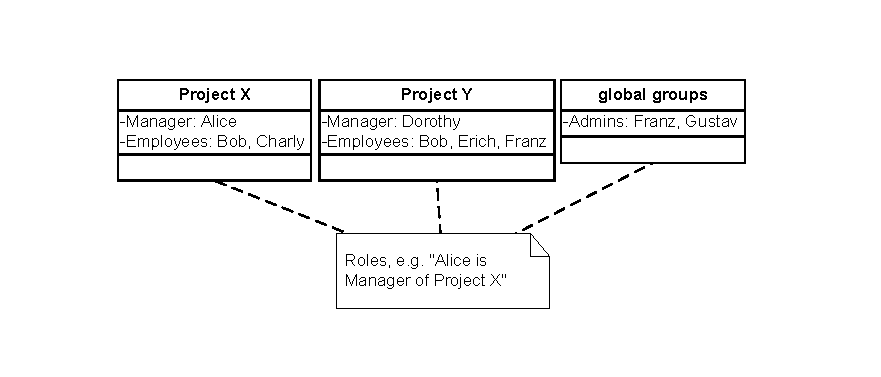
\includegraphics{images/Roles.pdf}
		\caption{Project roles}
		\label{project_roles}
	\end{center}
\end{figure}

Figure~\ref{project_roles} shows how the people are distributed on the projects:
Alice and Dorothy are managers, Bob is working on both projects, while Charly,
Erich and Franz are only working on one of the projects. Gustav is only an
administrator.

This leads to the following ultimate access rights for Alice, Bob, Erich and
Gustav:

\begin{tabular}{l|ll}
Person & Objects & Rights \\
\hline
Alice & Project X & READ,WRITE \\
	& Tasks of Project X & CREATE,DELETE,READ,WRITE \\
	& TimeRecords of Project X & CREATE,READ \\
	& TimeRecords with Owner==Alice & READ,WRITE \\
\hline
Bob & Project X and Y & READ,WRITE \\
	& Tasks of Project X and Y & READ,WRITE \\
	& TimeRecords of Project X and Y & CREATE,READ \\
	& TimeRecords with Owner==Bob & READ,WRITE \\
\hline
Erich & Project Y & READ,WRITE \\
	& Tasks of Project Y & READ,WRITE \\
	& TimeRecords of Project Y & CREATE,READ \\
	& TimeRecords with Owner==Erich & READ,WRITE \\
\hline
Gustav & ALL & ALL \\

\end{tabular}
